\documentclass{article}

\usepackage[main=english,vietnamese]{babel}
\usepackage[T1]{fontenc}
\usepackage[utf8]{inputenc}
\usepackage[sexy]{evan}
\usepackage{matchsticks}
\usepackage{wrapfig}
\usepackage{listings}

\newtheorem{hint}{Hint}

\title{Family trees}
\author{Nghia Doan}
\date{\today}

\begin{document}

\maketitle

Below you see an example of \textit{family tree}.
The circles denote female members and the triangles males.
\begin{center}
    \begin{minipage}[t]{6.5cm}
        \centering
        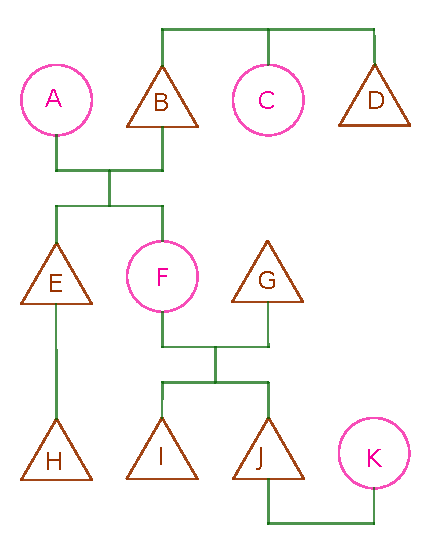
\includegraphics[width=4.5cm]{./svg/pdf/hc-2022-2-3-15-1.pdf}
    \end{minipage}
\end{center}

$A$ and $B$ are married, as are $F$ and $G,$ and $J$ and $K.$

$B, C,$ and $D$ are siblings, as are $E$ and $F.$
$E$ and $F$ are children of $A$ and $B.$

Similarly, the parents of $I$ and $J$ are $F$ and $G.$
$E$ is the father of $H.$

In addition, $A$ is the grandmother of $H, I,$ and $J,$
$F$ is the aunt of $H,$ and $C$ is the sister-in-law of $A.$

\newpage

\begin{example*}[Who are who]

    Inspector Jade asked six children to briefly introduce their brothers, sisters,
    and first cousins (cousins who share a grandparent.)
    She had to match the name of the child to each numbered position in the family tree
    with the responses as below. Note that the relations given are in local languague.
    \textit{Do not try to guess the genders of the children from the names. It might lead you to the wrong way.}

    \begin{center}
        \begin{minipage}[t]{7cm}
            Response from Binh:
            \begin{itemize}[topsep=0pt, partopsep=0pt, itemsep=0pt]
                \ii I have three \textit{arawa}: Kim, Minh, Thao
                \ii I have two \textit{surubu}: Oanh and Yen
            \end{itemize}
        \end{minipage}
        \hfill
        \begin{minipage}[t]{7cm}
            Response from Dinh:
            \begin{itemize}[topsep=0pt, partopsep=0pt, itemsep=0pt]
                \ii I have two \textit{surubu}: Oanh and Yen
                \ii I have one \textit{ere}: Binh
            \end{itemize}
        \end{minipage}
        \bigbreak
        \begin{minipage}[t]{7cm}
            Response from Kim:
            \begin{itemize}[topsep=0pt, partopsep=0pt, itemsep=0pt]
                \ii I have one \textit{arawa}: Dinh
                \ii I have one \textit{surubu}: Binh
            \end{itemize}
        \end{minipage}
        \hfill
        \begin{minipage}[t]{7cm}
            Response from Minh:
            \begin{itemize}[topsep=0pt, partopsep=0pt, itemsep=0pt]
                \ii I have one \textit{ere}: Yen
                \ii I have two \textit{arawa}: Dinh and Thao
            \end{itemize}
        \end{minipage}
        \bigbreak
        \begin{minipage}[t]{7cm}
            Response from Thao:
            \begin{itemize}[topsep=0pt, partopsep=0pt, itemsep=0pt]
                \ii I have two \textit{surubu}: Yen and Binh
                \ii I have two \textit{arawa}: Minh and Dinh 
            \end{itemize}
        \end{minipage}
        \hfill
        \begin{minipage}[t]{7cm}
        \end{minipage}
    \end{center}

\end{example*}

\begin{center}
    \begin{minipage}[t]{8cm}
        \centering
        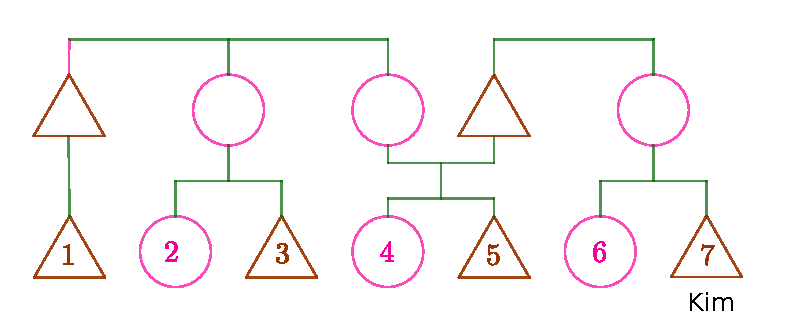
\includegraphics[width=8cm]{./svg/pdf/hc-2022-2-3-15-2.pdf}
    \end{minipage}
\end{center}

\begin{soln}
    From what Binh said, Binh has the same type of relations to three children.
    Thus, those cannot be Binh's sisters or brothers,
    and \textit{arawa} does not mean sister or brother.
    Only the child number $4$ or $5$ has three cousins in the same gender.

    Look at the cousins of the children $4$ or $5,$
    \textit{arawa} or \textit{suburu} rather related to the gender of the cousin
    than the gender of the cousin's father or the mother.
    Note that Binh is a \textit{suburu} to Kim and Kim is an \textit{arawa} to Binh.
    Thus, Binh and Kim are of opposite genders, so Binh is a girl.
    Hence, Binh is the girl number $4.$

    Therefore, Kim, Minh, and Thao are the children $1, 3,$ and $7,$
    and \textit{arawa} means \textit{male cousin(s).}
    Furthermore, Binh is a \textit{suburu} to Kim and Thao,
    in other words, she is a \textit{female cousin} to them.

    This means that Binh is not a \textit{suburu} to the boy $5.$
    Obviously, she is not an \textit{arawa} to anyone.
    Since she is an \textit{ere} to Dinh, Dinh must be her brother.
    Thus Dinh is the boy number $5.$
    
    Now, Thao must be the boy number $1$ because he has two female and two male cousins.
    That leaves Minh must be the boy number $3.$

    Yen is a \textit{ere} to Minh, so Yen is the girl number $2.$
    Finally, Oanh is the girl number $6.$

    The answer is $1-$Thao, $2-$Yen, $3-$Minh, $4-$Binh, $5-$Dinh, $6-$Oanh, $7-$Kim.  
\end{soln}

\end{document}